\section{Introduction}
In this section we will review the results of the asteroid search process on an increasingly difficult set of search tasks.
We will begin by developing two metrics we can use to compare a pair of orbital elements.
These metrics will be used to assess the quality of fitted elements when we have 
reason to believe they should match known orbital elements.
We can also use them to determine whether fitted elements match any asteroids in the known catalogue.
We begin by attempting to recover known orbital elements with a correct initialization but uninformed mixture parameters.
We work up to initializations with small and large perturbations of correct orbital elements.
Finally, we attempt a challenging search for orbital elements using random initializations.
We search separately on two subsets of the ZTF detections corresponding to known asteroids and unknown objects.

The model is highly successful recovering elements when initialized with even large perturbations.
Results from the random asteroid search are encouraging but less definitive.
I present 125 recovered orbital elements found by searching the known asteroid detections,
and 9 candidate orbital elements for new asteroids.
I state my conclusions, and lay out a program of future work on this topic.

\section{Comparing Candidate Elements to the Nearest Asteroid}
Before we review the results of our asteroid search experiments, it will be helpful to have in hand a notion of how closely two sets of orbital elements match.
In particular, we will test below whether or not we successfully recovered orbital elements when we started with them as an initial guess.
Answering this question requires that we have a useful metric on the space of orbital elements.

I spent a fair amount of time trying to develop such a metric.
While orbital elements are convenient for intuition and calculating orbits, there isn't an obvious distance metric we can put on them that makes a lot of sense.
Eventually I decided that the canonical way to compare two orbits is to compare the predicted vector of positions on a set of representative dates.
Logically this is hard to argue with, but it is somewhat computationally expensive compared to a computation that can be run directly on the elements.

The method \tty{nearest\_ast} searches the asteroid catalogue for the known asteroid whose orbit is closest to that predicted by the candidate elements.
It delegates its work to the function \tty{nearest\_ast\_elt\_cart}, which is defined in \tty{nearest\_asteroid.py}.
This function creates a set of 240 sample time points over 20 years spanning 2010 to 2030 sampled monthly.
The resulting table of positions for the asteroid catalog is fairly large, with a size of $733489 \times 240 \times 3$ (5.28E8 elements and about 2.11 GB using 32 bit floats).
Computing the nearest asteroid against $64$ candidate elements by brute force in TensorFlow would necessitate creating a tensor with 3.38E10 elements
or 135 GB of memory--two orders of magnitude too large for a high quality consumer grade GPU with $\sim 10$ GB of memory.
The nearest asteroid method is therefore forced to iterate through the elements one at a time, taking the norm of the difference against the table.
In one important optimization, the tensor of known asteroid positions in loaded into memory 
once as a TensorFlow constant to avoid recomputing it every time the function is called.

I also sought to develop a sensible metric of the distance between a pair of arbitrary orbital elements in the space of the orbital elements.
This is implemented in the same module with the function \tty{elt\_q\_norm} and \tty{nearest\_ast\_elt\_cov}.
The idea is to transform the elements to a Cartesian representation where they have a well behaved covariance matrix.
In particular, the goal is to find a deterministic transform of the elements that is distributed approximately as a multivariate normal.
Then the \href{https://en.wikipedia.org/wiki/Mahalanobis_distance}{Mahalanobis distance} is a natural metric on the transformed elements.
This process can be reviewed in the Jupyter notebook \tty{11\_nearest\_asteroid.ipynb}.
I initially tried working with the full empirical distribution to convert every orbital element to a percentile and then to a normally distributed $z$ score,
but the results didn't make any sense, so I dropped that approach.

Instead, I switched to a simpler approach and standardized variables so they would have mean 0 and variance 1.
I attempt to make them close to normal if possible, but without overfitting against the empirical distribution.
I standardized the log of the semi-major axis $a$ and directly standardized the eccentricity $e$.
\footnote{Even though this admits mappings from $z$ to eccentricities outside $[0,1]$, the mapping is only used in the direction
from a reported eccentricity $e$ to a transformed $e_z$ that is approximately normal.}
The quantity $\sin(i)$ was also also standardized.
Here is a summary of the mathematical transformations to create standardized 
(and hopefully approximately normal) variables from $a$, $e$ and $i$:
\begin{align*}
a_z &= \frac{\log(a) - \E[\log(a)]}{\sqrt{\Var[\log(a)]}} \\
e_z &= \frac{e - \E[e]}{\sqrt{\Var[e]}} \\
i_z &= \frac{\sin(i) - \E[\sin(i)]}{\sqrt{\Var[\sin(i)]}}
\end{align*}
The expectation and variance here are estimated using the sample mean and sample variance respectively.

Figure \ref{fig:ast_elt_standardize_a_e} shows visualizations comparing the hypothetical and empirical distributions of $a$ and $e$:
\begin{figure}[hbt!]
\begin{center}
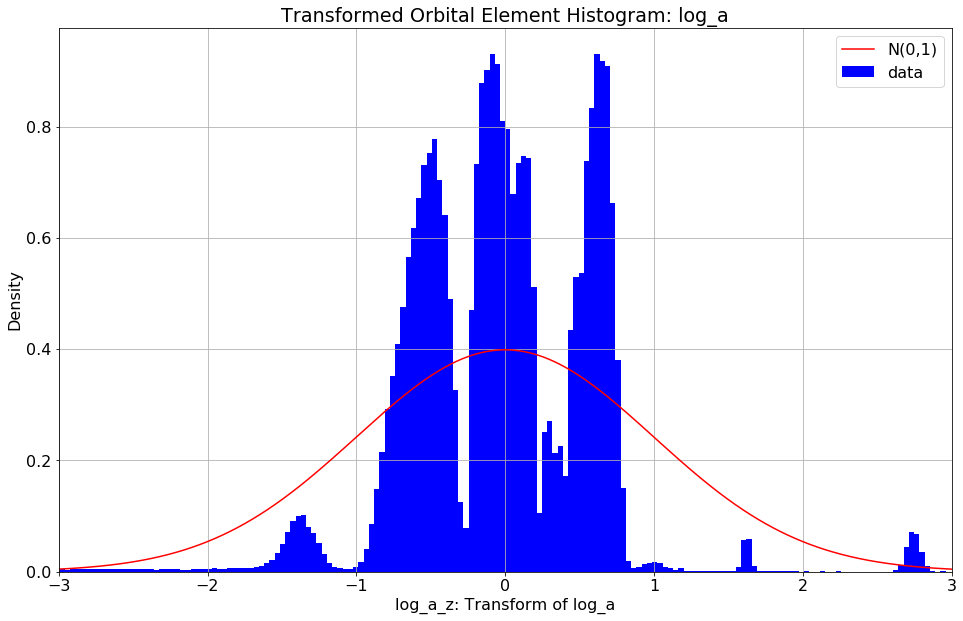
\includegraphics[width=0.8\textwidth]{../figs/elts_cov/log_a_z.png}
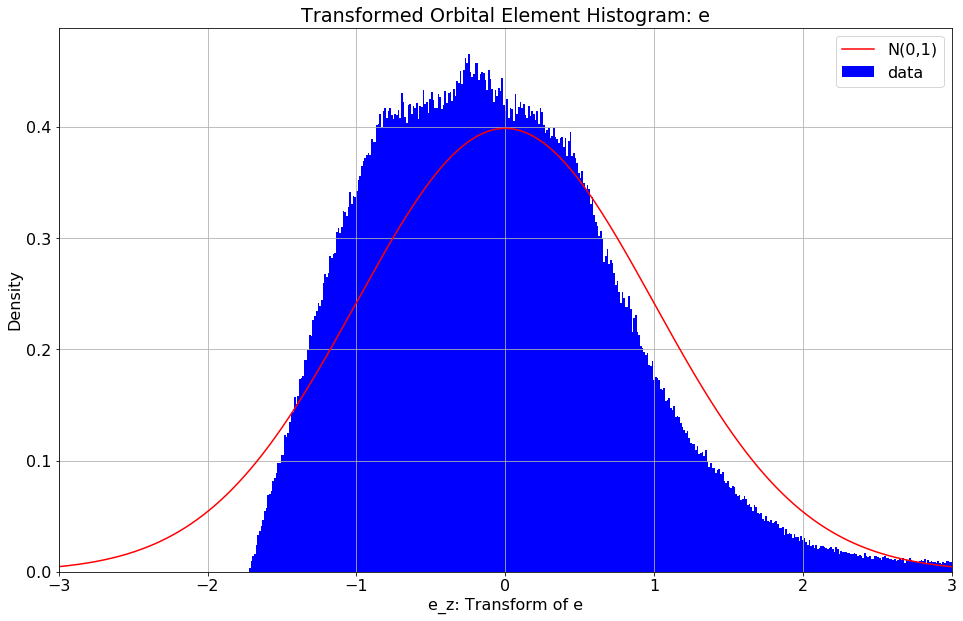
\includegraphics[width=0.8\textwidth]{../figs/elts_cov/e_z.png}
\end{center}
\caption[Transformations of $a$ and $e$ to Standardized Variables $a_z$ and $e_z$]
{Transformations of $a$ and $e$ to Standardized (and ``Approximately'' Normal?) Variables $a_z$ and $e_z$.}
\label{fig:ast_elt_standardize_a_e}
\end{figure}
\clearpage

We can inject $i$ into Cartesian space with only its sine because it is constrained to $[-\pi/2, \pi/2]$.
But the other three angles are unconstrained.  
They are handled identically.
I will take $\Omega$ as an example.
I transform $\Omega$ into \textit{two} variables, named \tty{cos\_Omega\_z} and \tty{sin\_Omega\_z}.
These are not transformed empirically, but using a theoretical distribution.
Let $x$ be the sine or cosine of one of $\Omega$, $\omega$ or $f$.
$x$ is mapped to a variable $z$ that is distributed approximately normal by applying the transformation
\begin{align*}
u &= \frac{1/2 + \arcsin(x)}{\pi} \\
z &= \Phi^{-1}(u)
\end{align*}
where $\Phi$ is normal CDF.
The simple idea is that if the angle $x$ distributed uniformly on the circle $[0, 2 \pi]$, 
then $u$ as defined here is uniform on $[0,1]$ and $z$ is standard normal.
Figure \ref{fig:elt_standardize_inc_omega} shows plots comparing the hypothetical and empirical distributions of $\sin(i)$ and $\sin(\Omega)$.
\begin{figure}[hbt!]
\begin{center}
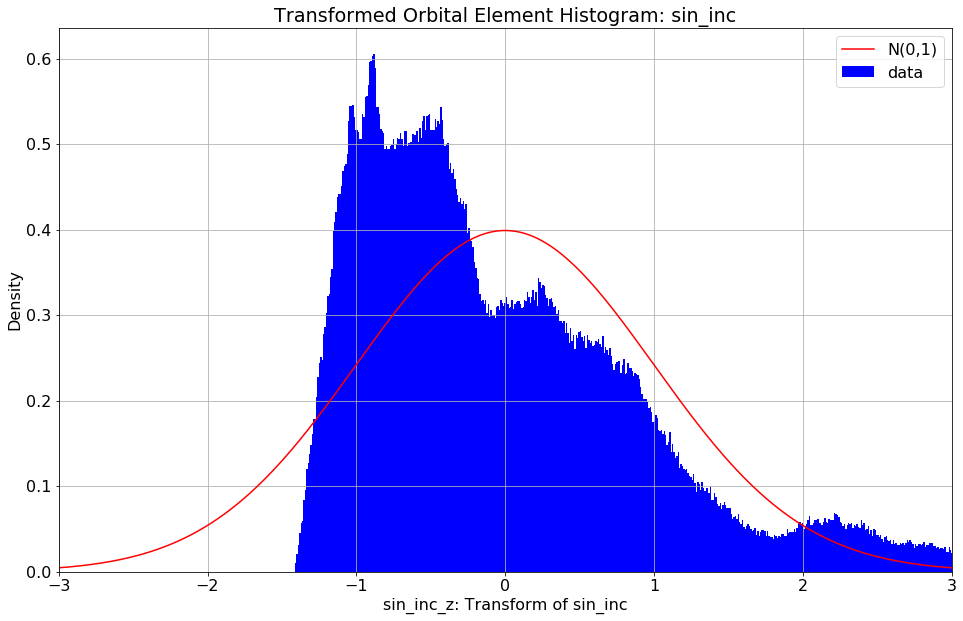
\includegraphics[width=0.8\textwidth]{../figs/elts_cov/sin_inc_z.png}
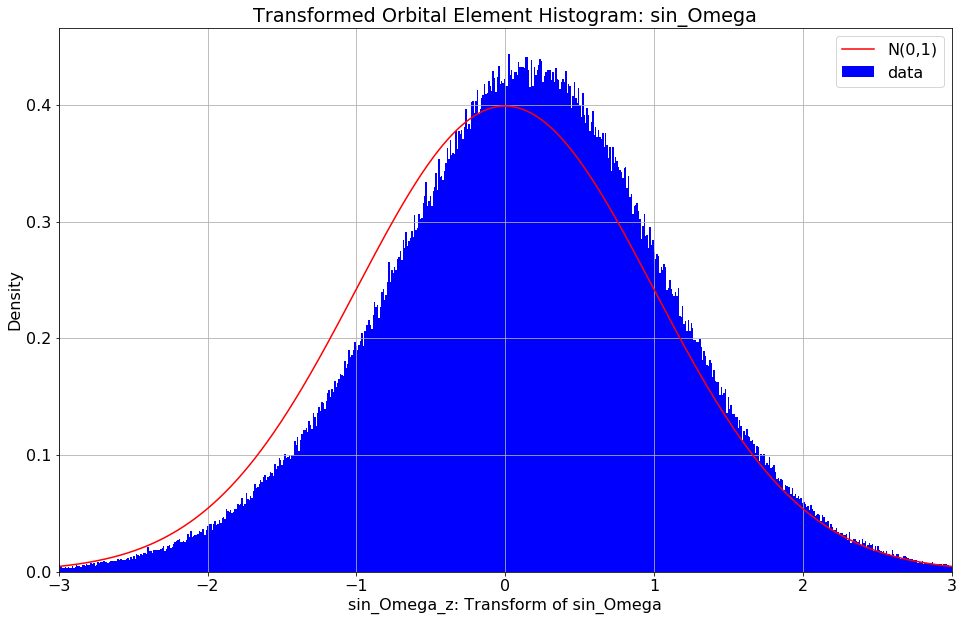
\includegraphics[width=0.8\textwidth]{../figs/elts_cov/sin_Omega_z.png}
\end{center}
\caption[Transformations of $\sin(i)$ and $\sin(\Omega)$ to Standardized Variables.]
{Transformations of $\sin(i)$ and $\sin(\Omega)$ to Standardized (and approximately normal) Variables.}
\label{fig:elt_standardize_inc_omega}
\end{figure}
Better results for $e$ and $i$ could be obtained by using the Beta distributions noted above, but for this purpose the simple standardization is adequate.
The plot shown for the transform of $\sin(\Omega)$ shows that it is very close to the theoretical distribution.
I generated analogous plots for the $\sin$ and $\cos$ of $\Omega$, $\omega$ and $f$ which are in the Jupyter notebook.
They are qualitatively similar to this one and all show excellent fits.

I have now given a recipe by which six orbital elements can be injected into $\R^{9}$.
Let $X$ be the $N \times 9$ matrix of transformed elements ($N$ = 733,489 is the number of asteroids).
The orbital elements are only very lightly correlated with each other, 
and so are the $X_j$ except for the tightly correlated pairs with the $\sin$ and $\cos$ of the same angle.
Next, using the Spectral Theorem, I find a $9 \times 9$ matrix $\beta$ such that the covariance matrix of $X \beta$  
(which also has shape $N \times 9$) is the $9 \times 9$ identity matrix.
The only wrinkle is that I assign importance weights to the 9 columns before building $X$ and computing $\beta$.
The importance weights are:
\begin{itemize}
\item 1.0 for $a_z$ and $e_z$
\item 0.5 for $i_z$
\item 0.1 for the $\sin$ and $\cos$ of $\Omega$, $\omega$ and $f$
\end{itemize}
These are admittedly qualitative judgments on my part. 
I initially only compensated for the double counting of $\Omega$, $\omega$ and $f$, 
but I noticed that relatively small differences in e.g. $\omega$ on a near circular orbit that hardly effected the shape of an orbit
were having a disproportionately large influence on the covariance score.

The covariance metric between two sets of orbital elements is $\epsilon_1$ and $\epsilon_2$ is defined by
$$ \norm{\epsilon_2 - \epsilon_1}_{\mathrm{cov}} = \norm{X_2 \beta - X_1 \beta} $$
The importance weights are rescaled so the diagonal of the covariance matrix sums to $1$ and a random pair of elements would have distance 1.
In practice I've observed that many pairs have norms far above $1$.
These calculations are also in \tty{nearest\_asteroid.py} and done by the 
functions \tty{elts\_to\_X\_cov}, \tty{calc\_beta}, \tty{elt\_q\_norm} and \tty{nearest\_ast\_elt\_cov}.
Now that we know what it means for two orbital elements to be ``close,'' 
we are ready for our first test: recovering unperturbed elements.

\section{Recovering the Unperturbed Elements of Known Asteroids}
\label{section_results_known_ast_unperturbed}

The first and easiest proof of concept for the search process is to see if the mixture parameters will converge correctly
when the search is initialized with correct orbital elements for asteroids that are well represented in the data,
but with ``neutral'' or uninformative mixture parameters.
I liken this test to a kid learning to swing a bat by trying to hit a ball sitting on a tee.
This test is demonstrated in the Jupyter notebook \tty{14\_asteroid\_search\_unperturbed.ipynb}.

It's worthwhile to follow through the steps to assemble the data to get familiar with how everything fits together.
These two lines of codes load the ZTF data observations associated with the nearest asteroid, and count hits by asteroid number:
\begin{lstlisting}[style=CodeSnippet]
ast_elt = load_ztf_nearest_ast()
ast_num, hit_count = calc_hit_freq(ztf=atf_ast, thresh_Sec=2.0)
\end{lstlisting}
The next few lines sort the asteroids in descending order by number of hits, 
and assemble a data frame of the orbital elements belonging to the 64 ``best'' asteroids.
The function \tty{asteroid\_elts} in \tty{candidate\_elements.py} provides a batch of candidate orbital elements
that exactly match known asteroids; it assigns an \tty{element\_id} matching the original asteroid number to make it easy
to check later if the fitted elements match the original.
The function \tty{load\_ztf\_batch} assembles the batch of ZTF observations within a threshold, 
here 2.0 degrees, of these candidate elements
\begin{lstlisting}[style=CodeSnippet]
elts_ast = asteroid_elts(ast_nums=ast_num_best[0:64])
ztf_elt = load_ztf_batch(elts=elts_ast, thresh_deg=2.0)
\end{lstlisting}

Reviewing the \tty{ztf\_elt} on screen we can see that there are 322,914 rows which include 10,333 hits:
an average of 161.5 hits per candidate element and 3.2\% of the total rows of data.
A call to \tty{score\_by\_elt} computes the $t$-score described earlier based on the mean and standard deviation of $\log(v)$.
This shows a mean $t$-score of +45.0, which is off the charts good.
It's interesting to see that a set of observations with 3.2\% hits and 96.8\% noise achieves such a good score.
This also puts into context the challenge of the search problem: 
we have an average of 5,045 detections within 2.0 degrees of each set of candidate elements,
of which 162 are hits and the remaining 4,883 are random detections belonging to other asteroids.
If we want a search process to detect asteroids with as few as 8 hits in the data, 
we will need a process selective enough to pick out just 0.16\% of the observations.

To initiate the search, we also need to choose our initial mixture parameters.
We set \tty{num\_hits} to $10$ and the resolution to $0.5$ degrees
\begin{lstlisting}[style=CodeSnippet]
elts_add_mixture_params(
	elts=elts_ast, num_hits=10, R_deg=0.5, thresh_deg=2.0)
\end{lstlisting}
Now that we have the candidate elements and the ZTF data frame, we are ready to instantiate the asteroid search model:
\begin{lstlisting}[style=CodeSnippet]
model = AsteroidSearchModel(
	elts=elts_ast, ztf_elt=ztf_elt, 
	site_name='palomar', thresh_deg=2.0)
\end{lstlisting}
Before we start training the model, we can get a plain text report or a visualization of the starting point.
I will omit these here. 
The report shows that at the start of training, all 64 elements are ``good'' with 5 or more hits,
and the overall mean log-likelihood is 3.13 and the mean number of hits is 162.7.
Here is an excerpt from the plain text model report at the end of training:\\
\begin{minipage}{\linewidth}
\begin{lstlisting}[style=CodeSnippet]
model.report()
Good elements (hits >= 5):  64.00

         \  log_like :  hits  :    R_sec : thresh_sec
Mean Good:  1096.95  : 162.55 :     3.01 :   165.95
Trained for 7808 batches over 122 epochs and 49 episodes (elapsed time 312 seconds).
\end{lstlisting}
\end{minipage}

Figures \ref{fig:TrainUnperturbed} and \ref{fig:TrainUnperturbedRes} illustrate the training progress.
We can see that the model is behaving as hoped.
It is gradually ratcheting the resolution parameter and scoring a high log-likelihood as it does so.
It does this without getting deked and polluting the originally correct orbital elements.
\newcommand{\subfigwidth}{0.5}
\begin{figure}[h]
\begin{subfigure}[t]{\subfigwidth\textwidth}
\centering
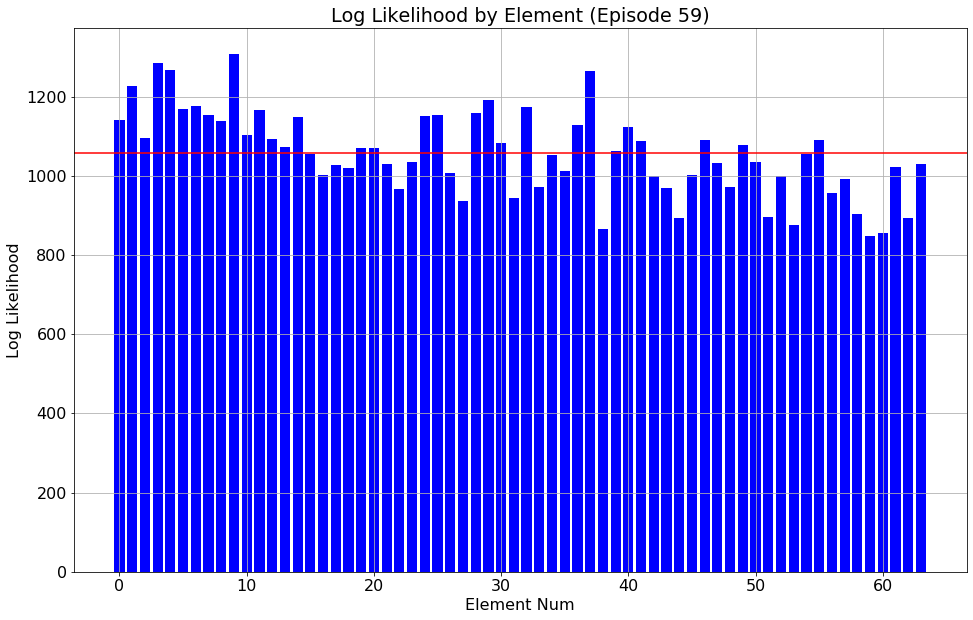
\includegraphics[width=\linewidth]{../figs/search_known/unperturbed/log_like.png}
% \caption{}
\end{subfigure}
\hfill
\begin{subfigure}[t]{\subfigwidth\textwidth}
\centering
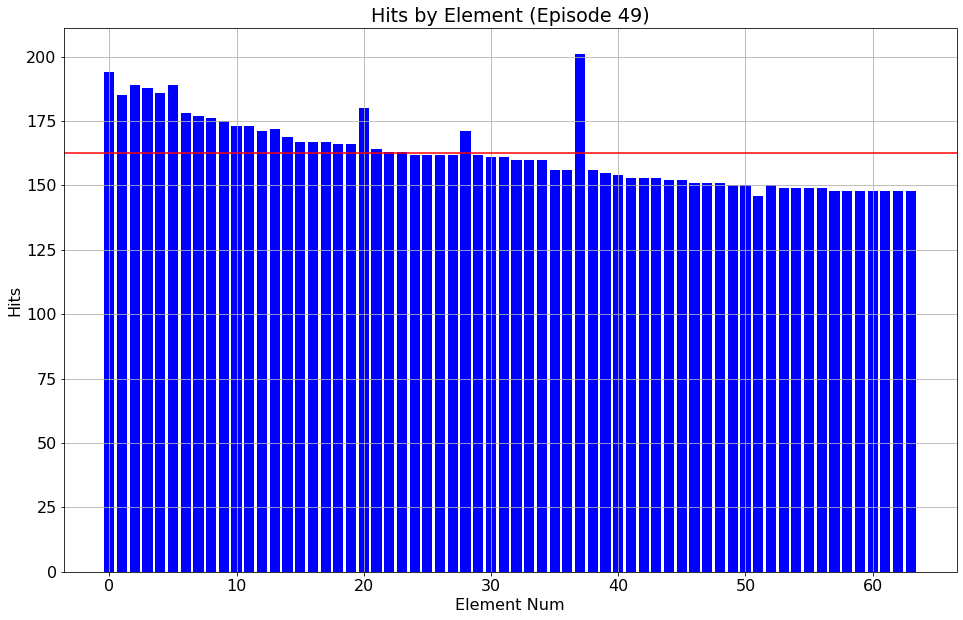
\includegraphics[width=\linewidth]{../figs/search_known/unperturbed/hits.png}
% \caption{}
\end{subfigure}
\medskip
\begin{subfigure}[t]{\subfigwidth\textwidth}
\centering
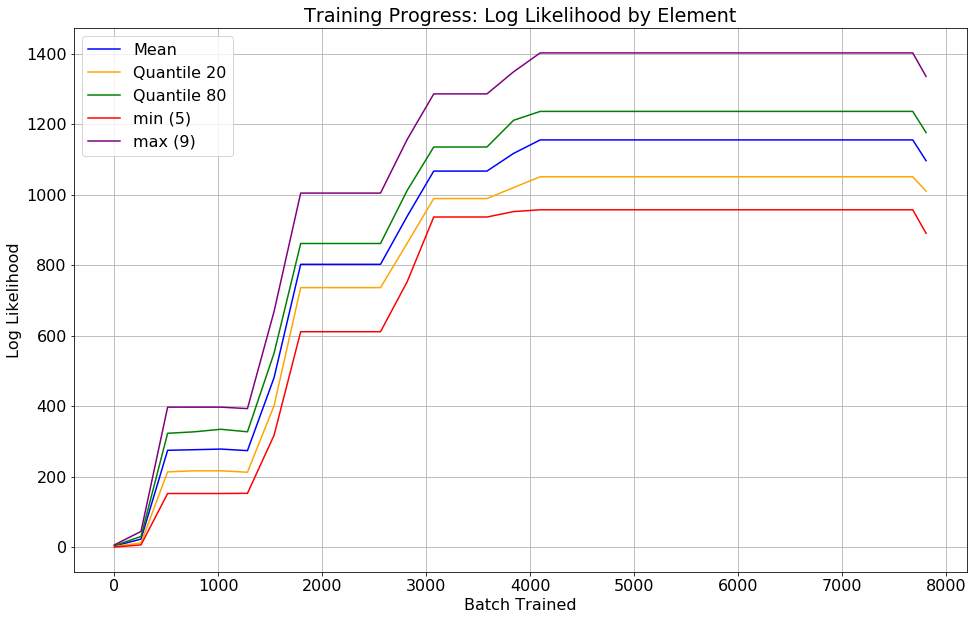
\includegraphics[width=\linewidth]{../figs/search_known/unperturbed/learning_curve_log_like.png}
% \caption{}
\end{subfigure}
\hfill
\begin{subfigure}[t]{\subfigwidth\textwidth}
\centering
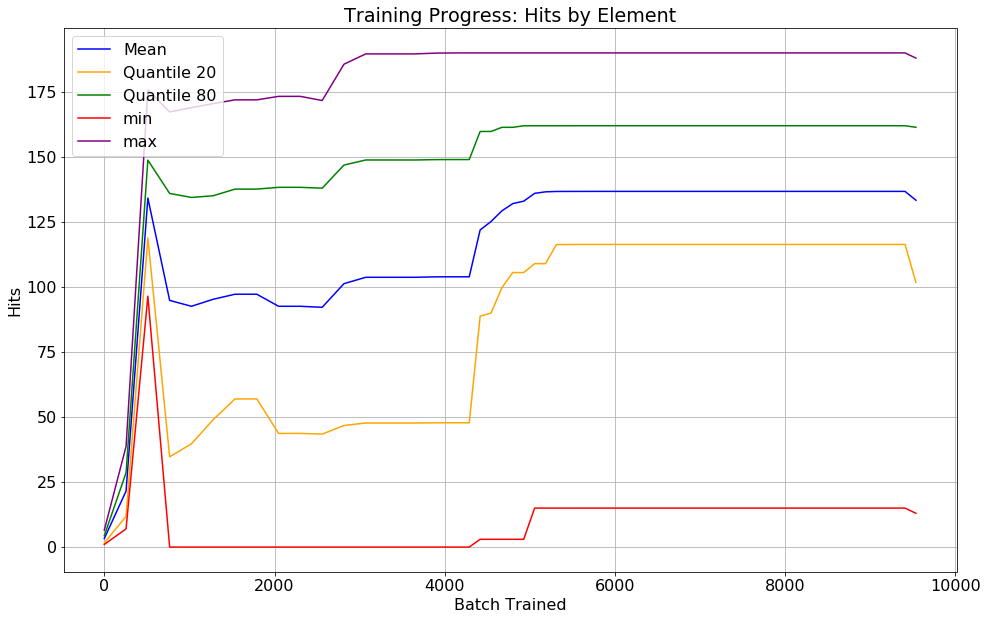
\includegraphics[width=\linewidth]{../figs/search_known/unperturbed/learning_curve_hits.png}
% \caption{}
\end{subfigure}
\caption[Training progress on 64 unperturbed orbital elements]
{Training progress on 64 unperturbed orbital elements.}
\label{fig:TrainUnperturbed}
\end{figure}
\begin{figure}[hbt!]
\begin{center}
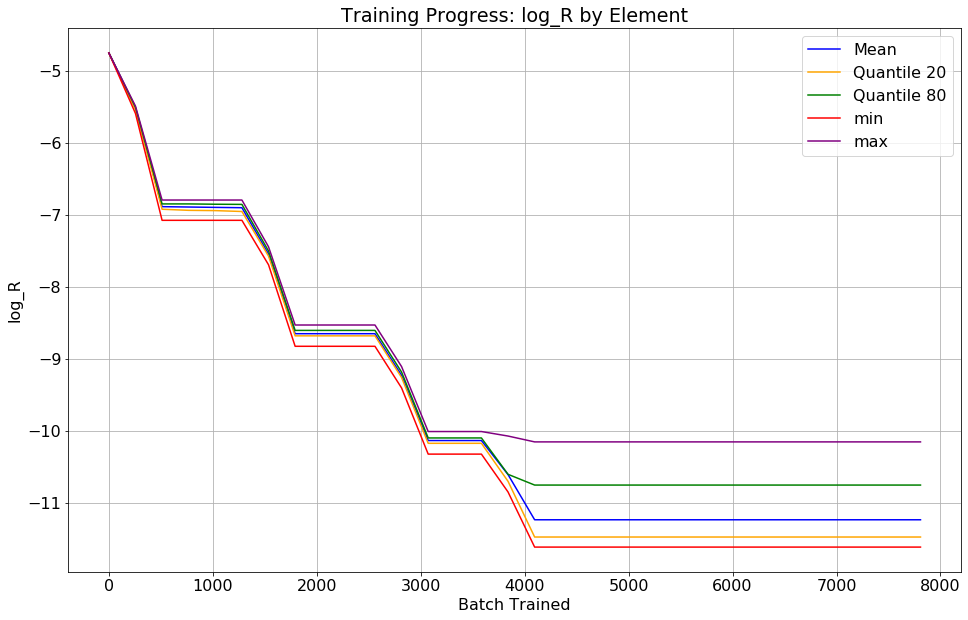
\includegraphics[width=0.7\textwidth]{../figs/search_known/unperturbed/learning_curve_log_R.png}
\end{center}
\caption[The resolution $R$ Decreases Monotonically when Training the Unperturbed Elements]
{The resolution $R$ Decreases Monotonically when Training the Unperturbed Elements.}
\label{fig:TrainUnperturbedRes}
\end{figure}
These are very happy diagnostics.  The log-likelihood averages over 1,000 and the hits average 160.
An earlier iteration of the training protocol that did not roll back training when hits were 
lost in an episode did considerably less well.

The diagnostics presented above work equally well for any set of candidate orbital elements,
whether or not they are ostensibly associated with a known asteroid.
In this case, we can further validate the results by comparing our fitted elements to the nearest asteroid
using the two metrics described in the previous section.
The simplest test is how many of 64 recovered elements have as their nearest asteroid the same asteroid used to initialize the elements.
The answer is 64: the fitting process ``tried'' to converge back to the right asteroid every time.
A more substantive question is how close did it come.  
Here are the summary statistics of two metrics:
\begin{itemize}
\item Mean distance in AU for 240 test points: $4.57 \times 10^{-8}$ (median over 64 elements)
\item Covariance Norm of elements: $5.70 \times 10^{-6}$ (geometric mean)
\end{itemize}
This is an excellent level of agreement.
The covariance norm is a good summary statistic, but may be hard to relate to astronomy.
The mean absolute error in the recovered $a$ is $4.3 \times 10^{-5}$ and in the recovered $e$ is $10^{-5}$.
Figure \ref{fig:UnperturbedNearAst} illustrates the distance in AU and covariance norm to the nearest (original) asteroid for all 64 candidate elements.
\begin{figure}[h]
\begin{center}
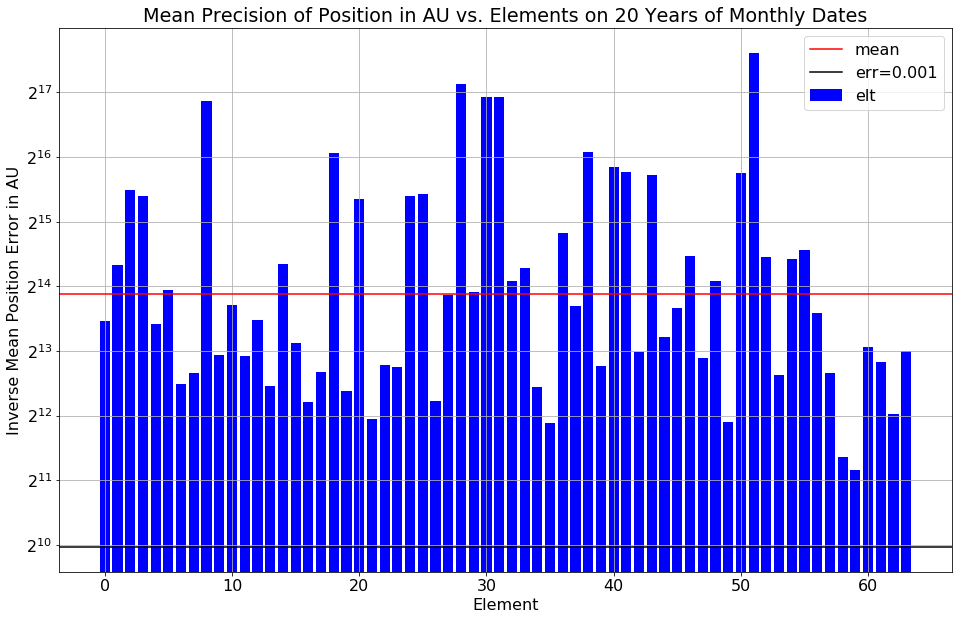
\includegraphics[width=1.0\textwidth]{../figs/search_known/unperturbed/near_ast_dist.png}
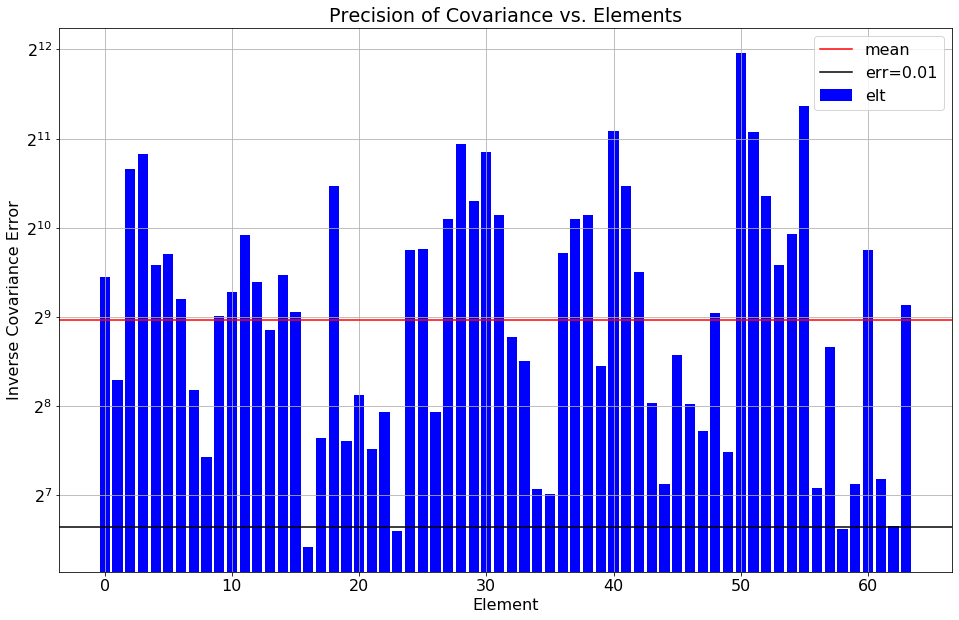
\includegraphics[width=1.0\textwidth]{../figs/search_known/unperturbed/near_ast_cov.png}
\end{center}
\caption[Two Metrics Comparing the Recovered Orbital Elements to True Elements]
{Two Metrics Comparing the Recovered Orbital Elements to the True Elements of the Asteroid in Question.\\
Both charts are plotted on a log scale with precision (reciprocal of the error) on the $y$ axis.\\
The geometric mean error is shown in red: $6.61 \times 10^{-6}$ AU and $2.00 \times 10^{-3}$ on the covariance norm.}
\label{fig:UnperturbedNearAst}
\end{figure}
Thanks to the one way ratchet that prevents it from losing hits once they acquired, 
the model can hit a tee ball out of the infield.
In the next section we will see how it fares against a moving target.
% \clearpage

\section{Recovering the Perturbed Elements of Known Asteroids}
\label{section_results_known_ast_perturbed}

\subsection{Small Perturbation}
The next experiment is similar to the previous one.
This time we will apply a small perturbation to the orbital elements in our initial guess.
If the last experiment was like hitting a tee ball, this one may be likened to hitting a ball gently pitched by your little league coach in batting practice.
The elements are perturbed using the function \tty{perturb\_elts} in \tty{candidate\_elements.py}.
The perturbation adds normally distributed random noise with the specified standard deviation
to $\log(a)$, $\log(e)$, and the four angles $i$, $\Omega$, $\omega$ and $f$.
The small perturbation shifts $\log(a)$ by $0.01$, $\log(e)$ by $0.0025$, $i$ by $0.05$ degrees,
and the the other angles by $0.25$ degrees.
A random seed is used for reproducible results.
The code to do this is
\begin{lstlisting}[style=CodeSnippet]
elts_pert= perturb_elts(elts_ast, sigma_a=0.01, sigma_e=0.0025, 
	sigma_inc_deg=0.05, sigma_f_deg=0.25, 
	sigma_Omega_deg=0.25, sigma_omega_deg=0.25,
	random_seed=42)
\end{lstlisting}
Last time the pre-training summary statistic based on $\log(v)$ showed a very positive $t$ score.
This time the $t$-score has dropped to $+3.71$, and the model has zero hits before it begins training.
Even this small perturbation is enough that the model is going to have to work quite a bit to recover the elements.
Here is the text report after sieving:
\begin{lstlisting}[style=CodeSnippet]
Good elements (hits >= 5):  42.00
         \  log_like :  hits  :    R_sec : thresh_sec
Mean Good:   798.24  : 117.50 :    36.06 :   779.79
Mean Bad :    42.97  :   0.64 :   266.21 :  2374.53
Trained for 15552 batches over 243 epochs and 105 episodes (elapsed time 751 seconds
\end{lstlisting}

Here are summary statistics for the run on the small perturbation of real asteroid elements:
\begin{itemize}
\item Successfully converged for 42 out of 64 candidate elements (65.6\%)
\item Hits on converged elements: 117.50 (mean)
\item Resolution on converged elements: 18.2 arc seconds (geometric mean)
\item Distance in AU to nearest asteroid: $2.58 \times 10^{-4}$
\item Covariance Norm to nearest asteroid: $1.22 \times 10^{-2}$
\end{itemize}
These results are not as strong as on the unperturbed elements, but the method is still clearly working.
It's coverged on almost two thirds of the candidate orbital elements.
The converged elements are fit well, averaging 117 hits at 18 arc seconds.
The distance to the nearest asteroid is $2.58 \times 10^{-4}$ AU, which is still very close and an excellent description of the orbit.
The nearest asteroid to the recovered elements matches the original asteroid on 48 out the 64 elements.

\begin{figure}[h]
\begin{subfigure}[t]{\subfigwidth\textwidth}
\centering
\includegraphics[width=\linewidth]{../figs/search_known/perturbed_small/log_like.png}
% \caption{}
\end{subfigure}
\hfill
\begin{subfigure}[t]{\subfigwidth\textwidth}
\centering
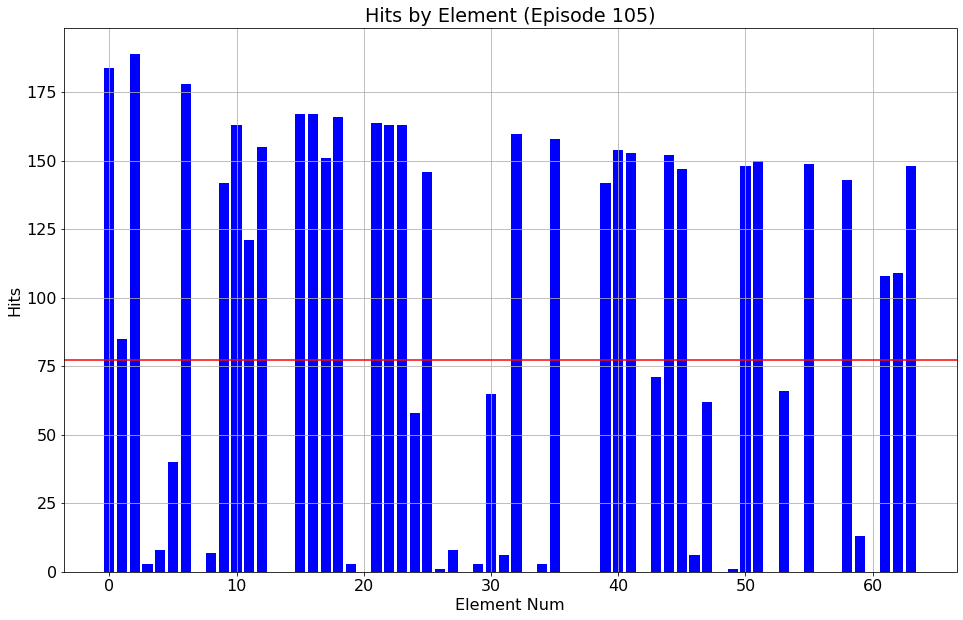
\includegraphics[width=\linewidth]{../figs/search_known/perturbed_small/hits.png}
% \caption{}
\end{subfigure}
\medskip
\begin{subfigure}[t]{\subfigwidth\textwidth}
\centering
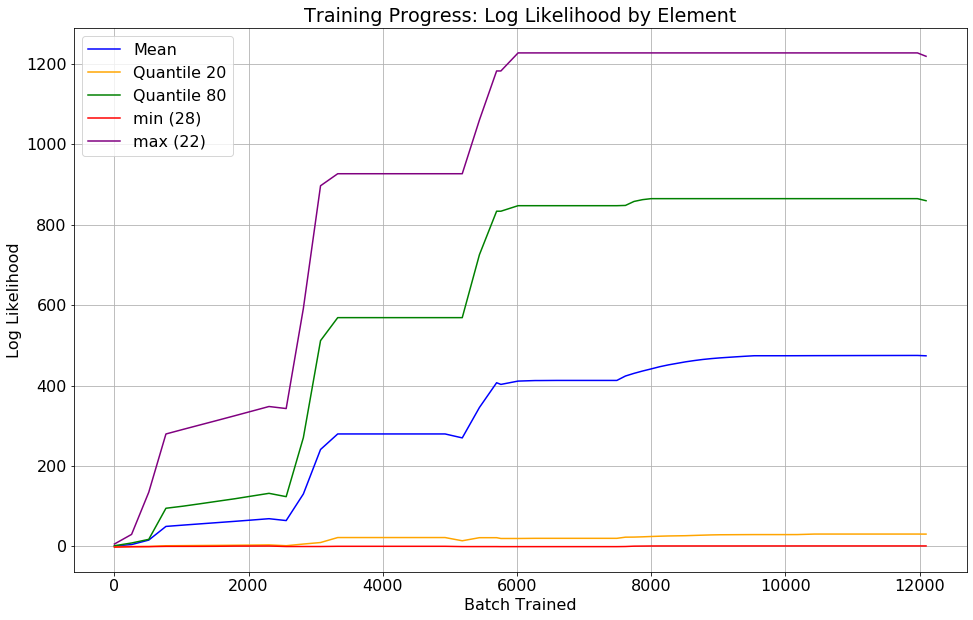
\includegraphics[width=\linewidth]{../figs/search_known/perturbed_small/learning_curve_log_like.png}
% \caption{}
\end{subfigure}
\hfill
\begin{subfigure}[t]{\subfigwidth\textwidth}
\centering
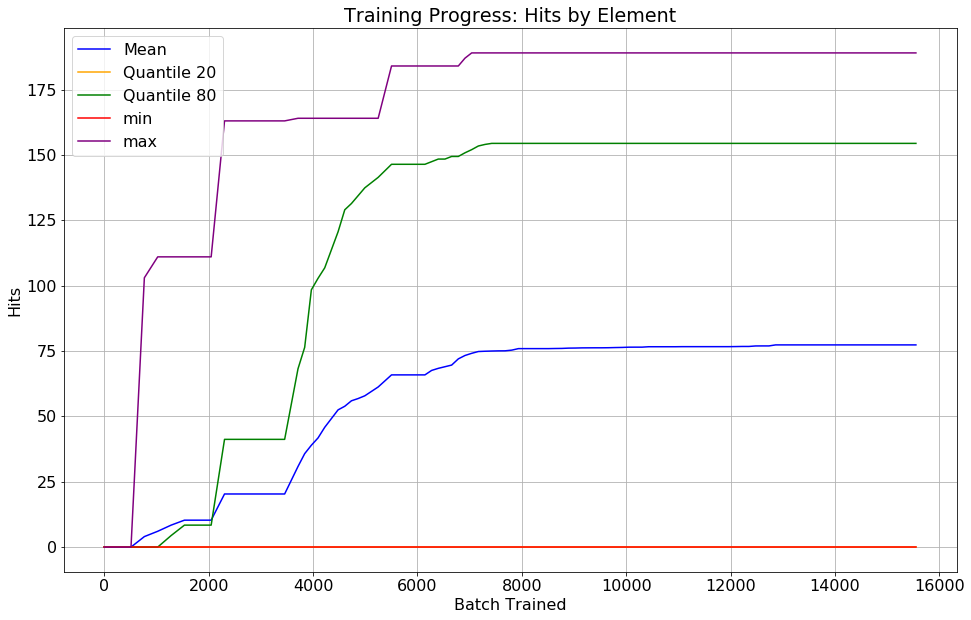
\includegraphics[width=\linewidth]{../figs/search_known/perturbed_small/learning_curve_hits.png}
% \caption{}
\end{subfigure}
\medskip
\begin{subfigure}[t]{\textwidth}
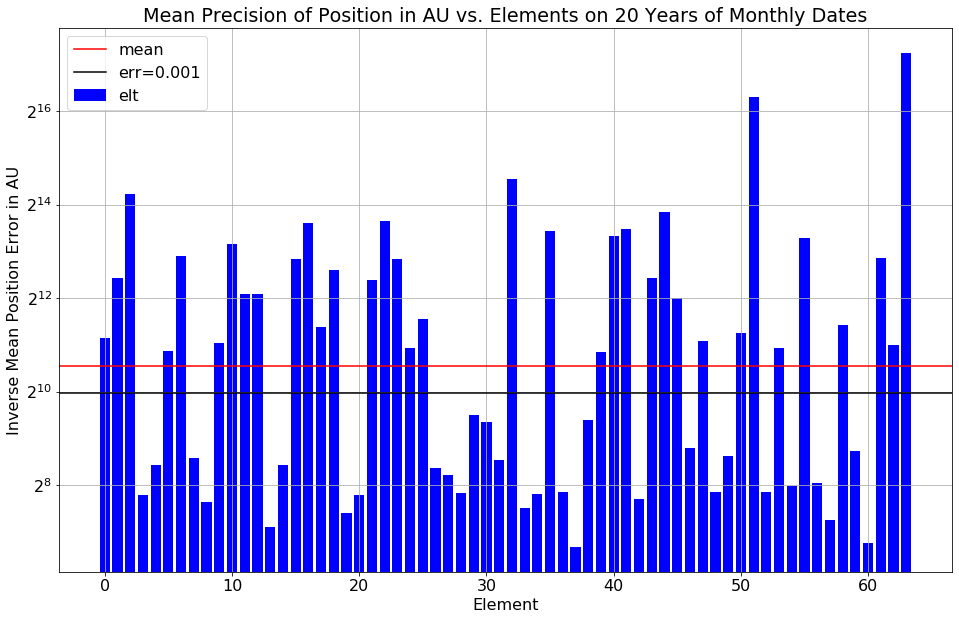
\includegraphics[width=1.0\textwidth]{../figs/search_known/perturbed_small/near_ast_dist.png}
\end{subfigure}
\caption[Training Progress on 64 Orbital Elements Initialized with Small Perturbations]
{Training Progress on 64 Orbital Elements Initialized with Small Perturbations from Real Asteroids.\\
42 of the 64 candidate elements converge, averaging 118 hits each.}
\label{fig:TrainingPerturbedSmall}
\end{figure}
\clearpage

\subsection{Large Perturbation}
In our third test, we will again start with perturbed orbital elements.
But this time, we will apply a larger perturbation, about five times larger.
This is a much harder task.  
To continue with the baseball analogy, it might be likened to facing a high school pitcher.
The perturbation size this time is 0.05 on $\log(a)$, $0.01$ on $\log(e)$, $0.25$ degrees on $i$, and $1.0$ degree on the other three angles.
While this might not sound like much at first, they are large perturbations.
In fact, they are so large they led me down a painful rabbit hole.
I repeatedly failed to recover the orbital elements of the original asteroids 
before I realized that the perturbations were large enough that in many cases, 
the nearest asteroid to the perturbed elements was no longer the original asteroid!
The results started to make much more sense when I compared each fitted element to the nearest real asteroid,
regardless of whether this matched the original source of the elements before perturbation.

Here is the text report after sieving:
\begin{lstlisting}[style=CodeSnippet]
Good elements (hits >= 5):  12.00
         \  log_like :  hits  :    R_sec : thresh_sec
Mean Good:   748.07  :  98.17 :    61.36 :  1178.94
Mean Bad :    30.35  :   0.58 :   261.02 :  2296.18
Trained for 13120 batches over 205 epochs and 72 episodes (elapsed time 533 seconds).
\end{lstlisting}

Here are summary statistics for the run on the large perturbation of real asteroid elements:
\begin{itemize}
\item Successfully converged for 12 out of 64 candidate elements (18.8\%)
\item Hits on converged elements: 98.2 (mean)
\item Resolution on converged elements: 32.4 arc seconds (geometric mean)
\item Distance in AU to nearest asteroid: $4.45 \times 10^{-4}$
\item Covariance Norm to nearest asteroid: $3.32 \times 10^{-2}$
\end{itemize}
This time we've only converged on 12 of the 64 orbital elements.
But the encouraging news is that when we have converged, the fit is still adequate.
The average hits are 98 and the resolution is 32.0 arc seconds.
The distance to the nearest asteroid is somewhat larger to the batch initialized with small perturbations, at $4.5 \times 10^{-4}$.
This is telling us something important: 
when the model starts from a good enough guess that it has a path in search space to a local maximum, it will converge to an adequate solution.
Starting from a poor initialization will reduce the probability of successful convergence, but it doesn't dilute the quality of the results.
\begin{figure}[h]
\begin{subfigure}[t]{\subfigwidth\textwidth}
\centering
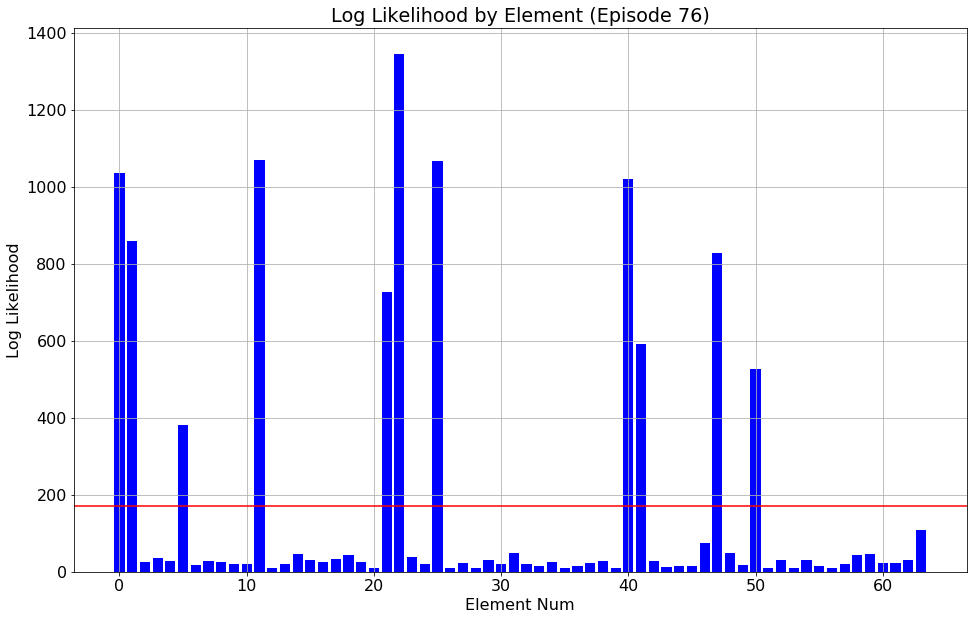
\includegraphics[width=\linewidth]{../figs/search_known/perturbed_large/log_like.png}
\end{subfigure}
\hfill
\begin{subfigure}[t]{\subfigwidth\textwidth}
\centering
\includegraphics[width=\linewidth]{../figs/search_known/perturbed_large/hits.png}
\end{subfigure}
\medskip
\begin{subfigure}[t]{\subfigwidth\textwidth}
\centering
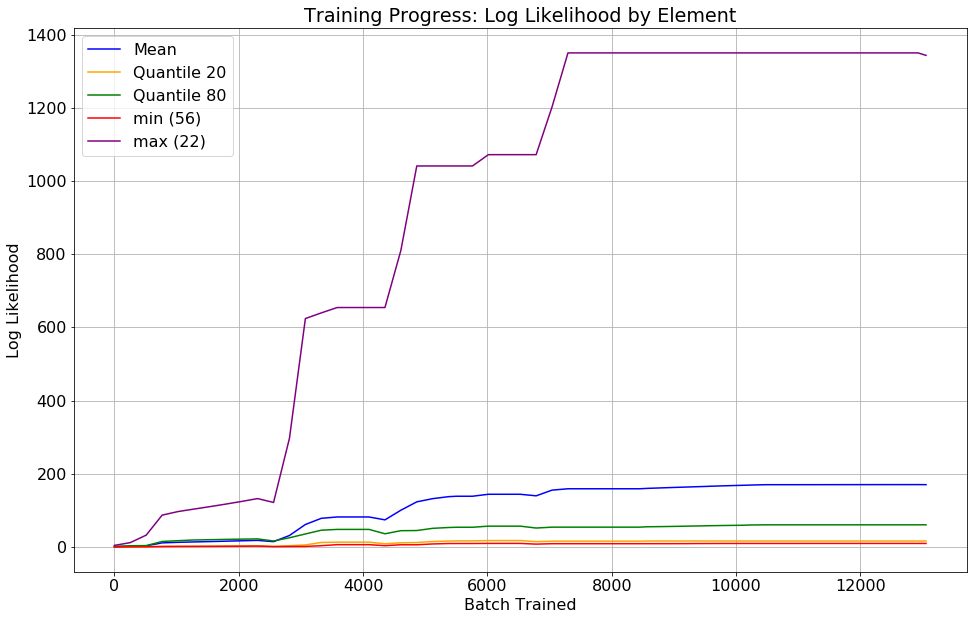
\includegraphics[width=\linewidth]{../figs/search_known/perturbed_large/learning_curve_log_like.png}
\end{subfigure}
\hfill
\begin{subfigure}[t]{\subfigwidth\textwidth}
\centering
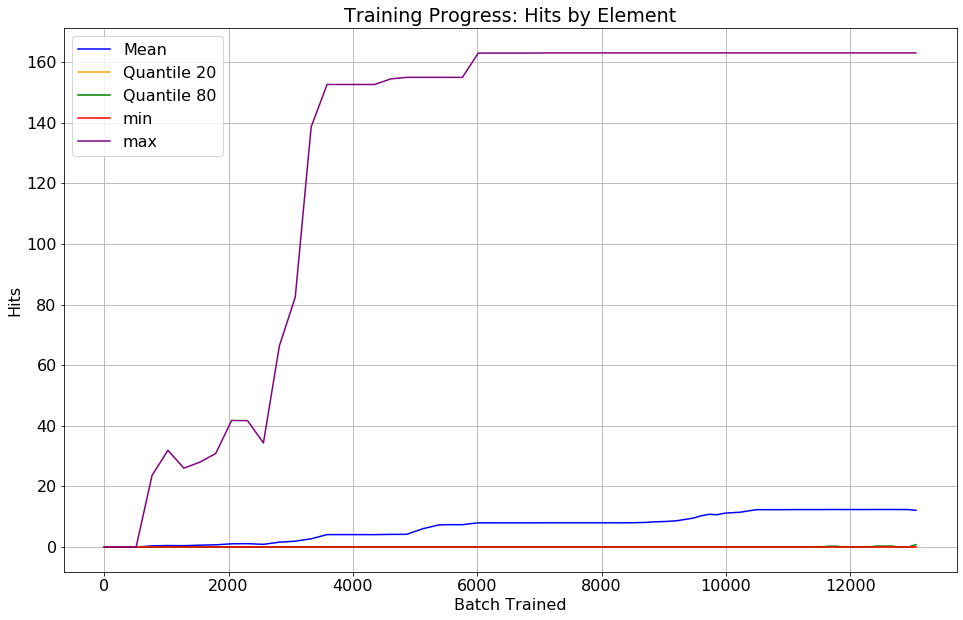
\includegraphics[width=\linewidth]{../figs/search_known/perturbed_large/learning_curve_hits.png}
\end{subfigure}
\medskip
\begin{subfigure}[t]{\textwidth}
\includegraphics[width=1.0\textwidth]{../figs/search_known/perturbed_large/near_ast_dist.png}
\end{subfigure}
\caption[Training Progress on 64 Orbital Elements Initialized with Large Perturbations]]
{Training Progress on 64 Orbital Elements Initialized with Large Perturbations from Real Asteroids.\\
12 of the 64 elements converge, averaging 98 hits.}
\end{figure}
\clearpage

\section{Searching for Known Asteroids with Random Initializations}
\label{section_results_known_ast_random}
Our final test case before searching for new asteroids is to attempt to recover asteroids in the known catalog, but without peeking at the answers.
I will now transition from small tests on a single batch of 64 candidate elements to analysis of the results of a large scale computational job.
We've entered the major leagues.
\footnote{Sadly, trying to fit asteroids with random initializations is a bit like facing Roger Clemens,
hoping to get hit by a pitch so you can get on base cheaply.}
The program \tty{asteroid\_search.py} can be run from the command line.
It searches against one of two subsets of the ZTF data set.
When run in ``known asteroids'' mode, the ZTF observations are filtered to include only the 3.75 million rows that are within 2.0 arc seconds of a known asteroid.
When run in ``unknown asteroids'' mode, it searches in the complement, the 1.95 million ZTF detections that are at least 2.0 arc seconds from a known asteroid.
The other arguments include the range of random seeds \tty{seed0} to \tty{seed1} and a stride to support parallelization.

This program was run on approximately 4096 random seeds against the known asteroids over the better part of a week.
Once a ZTF observation was associated with a set of candidate elements, it was subtracted from the data set so it would not be included in subsequent fits.
I filtered the results to those with at least 8 hits and a resolution of at most 20 arc seconds.
The results are reviewed in the Jupyter notebook \tty{19\_search\_known.ipynb}.
Since this was a search against known orbital elements, 
we can gauge the quality by measuring the distance of the recovered orbits to the nearest known asteroid.
Here are the summary statistics for the resulting fitted elements:
\begin{itemize}
\item 125 fitted orbital elements were found
\item Hits: 19.20 (mean)
\item Resolution: 9.3 arc seconds (geometric mean)
\item Distance to the nearest asteroid: $2.66 \times 10^{-3}$ AU (geometric mean)
\item Covariance Norm to the nearest asteroid: 0.73 (geometric mean)
\end{itemize}

\begin{figure}[h]
\begin{subfigure}[t]{\subfigwidth\textwidth}
\centering
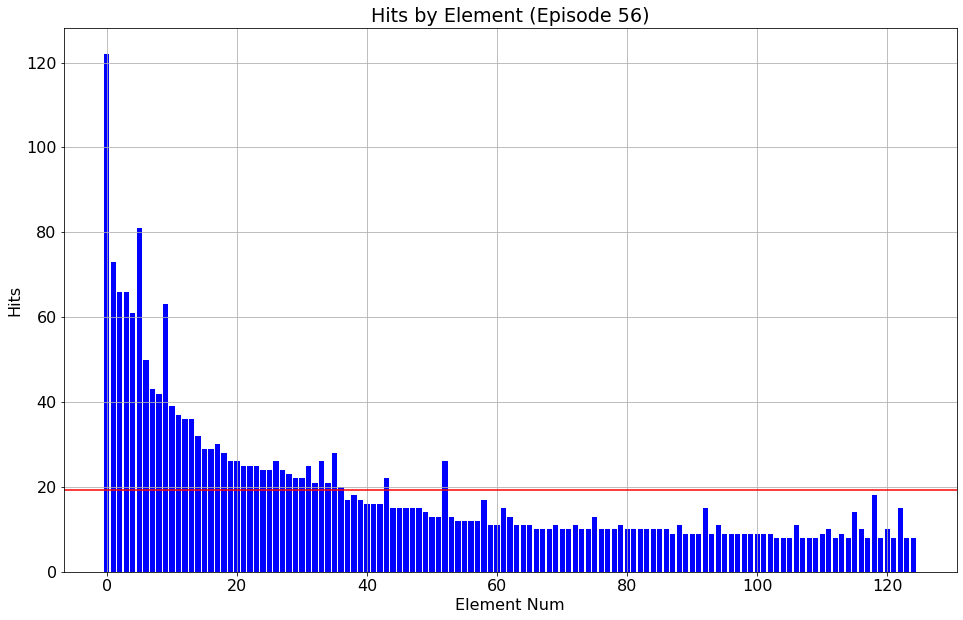
\includegraphics[width=1.0\textwidth]{../figs/search_known/random/hits.png}
\end{subfigure}
\hfill
\begin{subfigure}[t]{\subfigwidth\textwidth}
\centering
\includegraphics[width=1.0\textwidth]{../figs/search_known/random/log_like.png}
\end{subfigure}
\medskip
\begin{subfigure}[t]{\subfigwidth\textwidth}
\centering
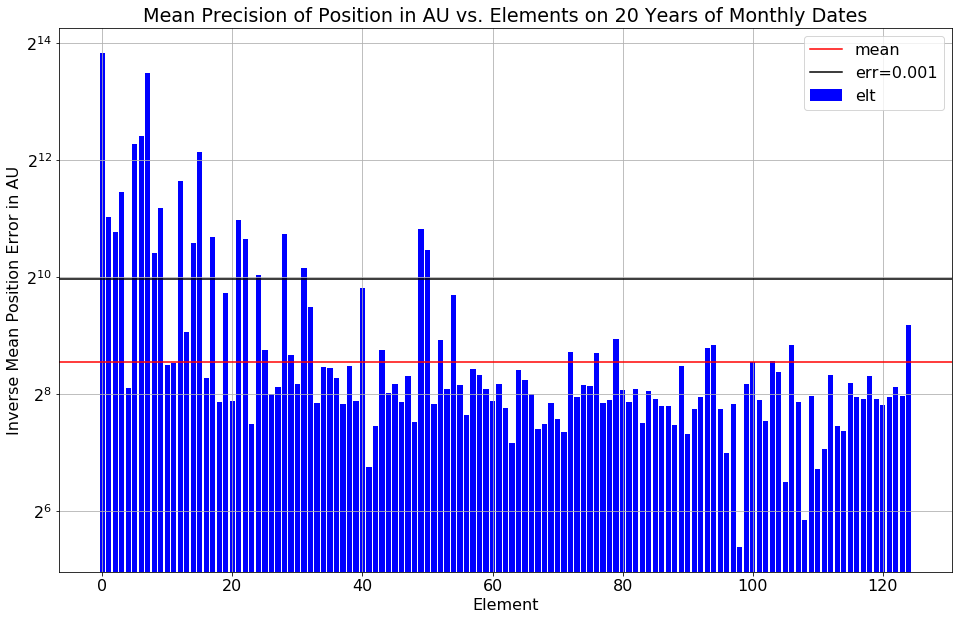
\includegraphics[width=1.0\textwidth]{../figs/search_known/random/near_ast_dist.png}
\end{subfigure}
\hfill
\begin{subfigure}[t]{\subfigwidth\textwidth}
\centering
\includegraphics[width=1.0\textwidth]{../figs/search_known/random/near_ast_cov.png}
\end{subfigure}
\caption[125 Orbital Elements Fitted to Observations of Known Asteroids]
{125 Orbital Elements Fitted to Observations of Known Asteroids.\\
The first row shows internal estimates of training quality: number of hits and log-likelihood.\\
The second row shows distance to the nearest known asteroid in mean distance of orbit and covariance metric.}
\label{fig:TrainRandomKnown}
\end{figure}

Figure \ref{fig:TrainRandomKnown} shows training results for the fitted elements.
The first row has the internal metrics number of hits and log-likelihood.
The second row has the comparison to the known asteroids.
I thought these results were respectable but not great.
I will need to significantly improve the initializations to get a higher yield.
The plots with the precision to the nearest asteroid are uneven.  
Some of these elements have clearly achieved excellent agreement with known asteroids, 
with positions accurate to $10^{-3}$ AU or better and covariance norms better than 0.1 (this is very close in orbital element space).
While there is room for improvement, I view this as a successful proof of concept that this technique can recover correct orbits of asteroids 
in the catalogue without peeking at the correct orbital elements.

\section{Presenting 9 New Asteroid Candidates}
\label{section_results_unknown_ast}
The search for new undiscovered asteroids is very similar to the search discussed in the previous section.
The only difference is that this time we limit the search to the subset of 
1.95 million ZTF observations more than 2.0 arc seconds away from any known asteroid.
A search was carried out starting from 4,096 random seeds, taking about 5 days running on 4 GPUs in parallel.
This search identified 9 candidate orbital elements that achieved at least 8 hits within 10 arc seconds
and a converged resolution less than 20 arc seconds.
These are the same criteria used to select the ostensibly high quality recovered orbital elements of known asteroids presented in the last section.

\begin{figure}[h]
\begin{center}
\includegraphics[width=1.0\textwidth]{../figs/search_unknown/candidate_elements_dataframe.png}
\end{center}
\caption{Orbital Elements of 9 Candidate Asteroids.}
\label{fig:CandidateOrbitalElements}
\end{figure}
Figure \ref{fig:CandidateOrbitalElements} shows the candidate orbital elements.
Here are the summary statistics for the new asteroid candidates:
\begin{itemize}
\item 9 fitted orbital elements were found
\item Hits: 9.11 (mean)
\item Resolution: 5.3 arc seconds (geometric mean)
\item Distance to the nearest asteroid: $4.10 \times 10^{-3}$ AU (geometric mean)
\item Covariance Norm to the nearest asteroid: 1.10 (geometric mean)
\end{itemize}

\begin{figure}[h]
\begin{subfigure}[t]{\subfigwidth\textwidth}
\centering
\includegraphics[width=1.0\textwidth]{../figs/search_unknown/hits.png}
\end{subfigure}
\hfill
\begin{subfigure}[t]{\subfigwidth\textwidth}
\centering
\includegraphics[width=1.0\textwidth]{../figs/search_unknown/log_like.png}
\end{subfigure}
\medskip
\begin{subfigure}[t]{\subfigwidth\textwidth}
\centering
\includegraphics[width=1.0\textwidth]{../figs/search_unknown/near_ast_dist.png}
\end{subfigure}
\hfill
\begin{subfigure}[t]{\subfigwidth\textwidth}
\centering
\includegraphics[width=1.0\textwidth]{../figs/search_unknown/near_ast_cov.png}
\end{subfigure}
\caption[Fit Quality for 9 New Asteroid Candidate Orbital Elements]
{Fit Quality for 9 New Asteroid Candidate Orbital Elements.\\
The first row shows internal estimates of training quality: number of hits and log-likelihood.\\
The second row shows distance to the nearest known asteroid in mean distance of orbit and covariance metric.}
\label{fig:TrainUnknown}
\end{figure}

Figure \ref{fig:TrainUnknown} shows the fit quality and distance to the nearest asteroid, as with the known asteroid search.
These results are encouraging but not quite as definitive as I had hoped.
The convergence with 9.1 hits to a resolution of 5.3 arc seconds strikes me as excellent.
A RA/Dec observation has 2 degrees of freedom, so a collection of 6 free parameters (the orbital elements)
is matching 18 degrees of freedom of data at a composite tolerance of about 5 arc seconds.
Log-likelihood scores in the range of 40-60 lead me to believe to me that this process 
has successfully identified collections of observations that are highly likely to belong to the same or perhaps related objects,
and that it has fitted orbital elements to the observations to a good tolerance.

The news is not quite as a good when I look at the distance to the nearest asteroid in the catalogue.
I had hoped to present compelling evidence that the recovered elements trained against the
known asteroid subset of the ZTF detections were much closer to the nearest known asteroid than these elements.
While it is true that the these elements are further away by a factor of 1.54 in mean distance,
and 1.51 on the covariance norm, that is not a big margin.
I have to admit here the possibility that while these elements correspond to a real object,
they might have converged to elements close to those of a known asteroid.
When I set up the training to exclude detections near to known asteroids,
I thought it was unlikely that it would converge to a known asteroid, and I still believe that to be true.
There is a possibility that these candidates might be better interpreted as proposed revisions to the
orbital elements of nearby asteroids than as new, undiscovered objects.

Figure \ref{fig:ZtfHits} shows the ZTF hits the search process has associated with each set of candidate elements.
We can gain understanding by paying close attention to the ObjectID column.
These are provisional assignments by ZTF indicating that multiple detections are likely to belong to the same object.
Take four example candidate elements in turn.  \\
Element \tty{178421} is stringing together four detections of object \tty{ZTF18aboluox} and 4 detections of object \tty{ZTF18acewaex}.
They were seen 433 days apart.  
The magnitudes are very different, so this is probably a spurious connection between two different objects with compatible orbits.\\
Element \tty{3308} is piecing together 6 detections of \tty{ZTF18abtpdzg} and 2 detections of \tty{ZTF18abspkzw}.
These detections were made 193 days apart.
The magnitudes of these are compatible, making it far more plausible that this is a legitimate connection between 
two sets of detections that may not have been made previously. \\
Element 191915 is again stringing together 6 + 2 detections of different objects (\tty{ZTF18abtxgd} and \tty{ZTF19abtsqmn})
made 469 days apart.  The magnitudes are all compatible.  
This too seems likely to be a legitimate and novel connection between different sets of detections. \\
Element \tty{170789} is an example of a fit made by stringing together just one set of detections
made at similar times.  All of the detections are of the same ZTF object \tty{ZTF17aaqwwg} made on the same date,
indeed made in a time span of only 55 minutes.
The model has independently matched the conclusion of the ZTF classifier that all 8 detections belonged to the same object.
\begin{figure}[h]
\begin{subfigure}[t]{0.45\textwidth}
\centering
\includegraphics[width=\linewidth]{../figs/search_unknown/ztf_hits_178421.png}
\end{subfigure}
\hfill
\begin{subfigure}[t]{0.45\textwidth}
\centering
\includegraphics[width=\linewidth]{../figs/search_unknown/ztf_hits_3308.png}
\end{subfigure}
\bigskip
\begin{subfigure}[t]{0.45\textwidth}
\centering
\includegraphics[width=\linewidth]{../figs/search_unknown/ztf_hits_191915.png}
\end{subfigure}
\hfill
\begin{subfigure}[t]{0.45\textwidth}
\centering
\includegraphics[width=\linewidth]{../figs/search_unknown/ztf_hits_170789.png}
\end{subfigure}
\caption[ZTF Hits Associated with 4 of the New Asteroid Candidate Elements]
{ZTF Hits Associated with 4 of the New Asteroid Candidate Elements.}
\label{fig:ZtfHits}
\end{figure}
While I would like to marshal further evidence that these candidate elements belong to new objects,
I find the detailed analysis of the claimed series of ZTF hits to be persuasive and encouraging.
This search process is clearly identifying plausible connections between related detections 
by brute force analysis of their location in the sky.

\section{Conclusion}
\label{search_conclusion}
In this thesis I have presented a novel technique for learning orbital elements of asteroids from telescopic data: searching in the space of orbital elements.
This approach has significant theoretical advantages over methods that rely on stringing tracklets together, which suffer from a combinatorial explosion.
I have demonstrated a working prototype and shown that it can converge well to correct orbital elements from a suitable initialization.
This prototype also illustrates how to perform large scale and efficient astrometric computations on GPUs using TensorFlow,
which is a second potentially novel contribution.
I have further demonstrated that even naive random initializations are sufficient to reidentify up to 125 known asteroids, albeit to varying degrees of quality.
Finally, I have proposed candidate orbital elements for up to 9 previously unknown asteroids.
By analyzing the details of the ZTF detections associated with each candidate element,
I have provided anecdotal evidence that the search is identifying detections that plausibly belong to the same object.

\section{Future Work}
\label{section_future_work}

\subsection{Intelligent Initialization of Candidate Elements}
\label{subsection_intelligent_initialization}
When I first conceived this project, I intended to devote substantial time to formulating intelligent initializations of the candidate orbital elements.
The random orbital elements were intended as a quick and dirty placeholder to get the system up and running.
\footnote{The ubiquitous operating system DOS was named ``Disk Operating System.''
It was built around an operating system that was called QDOS, for ``Quick and Dirty Operating System.''
The marketing department at Microsoft was savvy enough to realize that they needed a new etymology 
for their OS, so they rebranded it DOS.
See \href{https://en.wikipedia.org/wiki/86-DOS}{Wikipedia - 86-DOS}.
I share this anecdote to illustrate that quick and dirty solutions in computing often last longer than one might have hoped.}
Due to the looming deadline I have had to defer that to future work.
The results presented for perturbed orbital elements were very encouraging, showing excellent convergence.
If we can identify a set of candidate orbital elements that are close to real ones, this process should efficiently grab
all the other detections in the data set that are consistent and combine them.

The ZTF data set includes an ObjectID column that represents a preliminary assessment of which detections are related.
A straightforward method for initializing candidate orbital elements is to take these classifications at face value.
For each ObjectID, take the collection of $k$ detections and use a traditional technique (e.g. least squares fitting) to find orbital elements consistent with them.
In fact, the existing \tty{AsteroidSearch} class provides most of the code required to do this.
To adapt it to this problem, we would ignore the mixture parameters and minimize the least squares loss rather than maximizing the log-likelihood.

Here is a more ambitious idea for intelligent initialization.
By looking at the subset of ZTF detections within 2.0 arc seconds of a known asteroid, we can generate a large collection of training data
of pairs of ZTF detections that we are highly confident belong to the same object.
We can randomly sample other pairs of ZTF detections, and use the two data sets to train a binary classifier to predict 
the probability that a pair of ZTF detections belong to the same object.
This classifier could be used to come up with tracklets that might not have the same ObjectID.
An additional classifier might also be trained to try to extend a tracklet with a third detection.
Each detection has 2 degrees of freedom, and an orbital element has 6.
So a single tracklet allows us to sample a 2D space of candidate element consistent with it,
while three or more detections should in theory give us a uniquely determined initialization point.

\subsection{Incorporating Additional Data}
The method presented doesn't use anything special about the ZTF data set besides for the filtering of likely asteroid detections.
While the ZTF data set is excellent, it only dates back effectively to the middle of 2019.
An obvious step to improve these results would be to bring in a second major data source.
I would probably start with Pan-STARRS.
Ideally I would like to identify a subset of detections that have already been classified as likely to be near Earth objects.
Failing that, we could start with all Pan-STARRS data; remove bogus detections with a real-bogus classifier;
and subtract out detections of stars and galaxies by using the catalogue of their known positions in the sky.
The code would need to be changed in some places, but the change would not be major.

\subsection{Incorporating Magnitude}
I developed code in the \tty{AsteroidSearch} model to predict the magnitude of a detection using the H-G model.
I also had a version of the log-likelihood that incorporated a joint probability density on both direction and magnitude.
The theoretical advantages of an estimation framework that incorporates magnitude are substantial.
The model will be much less likely to make spurious connections of detections with compatible orbits
that can't be the same object because they have different magnitudes.
An added benefit is that the fitting procedure would give estimates for $H$ and $G$.
Unfortunately, I was not able to get the fitting process to converge well when I included the magnitude in the joint probability.
As time drew short, I was forced to remove it from the model presented here and punt it to future work.
I am highly optimistic that given enough time, this can be made to work and will sharpen the results.

\subsection{Rebuilding the Known Asteroid Catalogue}
If the three improvements above are made, I believe there is a good chance this model might be able to rebuild a large portion of the known asteroid catalogue.
We saw that just seven months of ZTF data included over 100,000 asteroids with 10 or more hits, encompassing 13.6\% of the known catalogue.
The random initialization is not remotely up to the task of recovering all these elements, but with intelligent initialization alone we would be in the game.
I think it would be a powerful proof of concept if we could run a program that would crunch through tens or hundreds of millions of detections and
generate an output with large overlap against the known asteroids.
At a minimum, it would validate a single automated procedure that could also detect new objects.
It might also allow us to gradually improve the quality of the data in the known asteroid catalog.

The ultimate goal of this body of work could be to build a single, fully automated computational pipeline for asteroid classification.
Telescopic detections from multiple surveys would go in, optionally alongside snapshots of the known asteroid catalogue.
The output would include an association of detections to known objects; revisions to the catalog where necessary; 
and proposed additions to the catalogue when supported by new detections.